\section{Results}\label{sec:results}

The analyses use \res{nBMused} building-month-tariff cells after the exclusion rule of Section~\ref{sec:model}. Unless stated otherwise, results refer to tariff T1, the demand-charge tariff.

\subsection{Accuracy does not rank forecasters by value (H1)}

Executed open loop, the ranking of the five forecasters by MAE did not agree with their ranking by captured share. The mean over buildings of the per-building Kendall $\tau$ was $\res{honeMean}$ (median $\res{honeMedian}$; positive in \res{honePos}\% of buildings; $t=\res{honeT}$, $p=\res{honeP}$; sign test $p=\res{honePsign}$), so the primary hypothesis is not supported; if anything, the more accurate forecaster tended to capture slightly less. Ranking by RMSE instead gave $\tau=\res{honermseMean}$ ($p=\res{honermseP}$), and the \res{honenofillN} buildings without filled gaps gave $\tau=\res{honenofillMean}$ ($p=\res{honenofillP}$). With the guarded controller (H1b, secondary) the agreement was positive but weak: $\tau=\res{honebMean}$, positive in \res{honebPos}\% of buildings ($p=\res{honebP}$).

An exploratory count makes the size of the gap concrete. In a building-month, the forecaster with the lowest MAE was also the one with the largest captured share in \res{mostAccOpen}\% of cases with open-loop execution and \res{mostAccGuard}\% with the guard. If accuracy and value were unrelated the figure would be 20\%; it is lower because the least accurate forecaster was usually the most valuable (Section~\ref{sec:res-errors}).

\subsection{The controller matters more than the forecaster (H4)}

\begin{figure}[t]
\centering
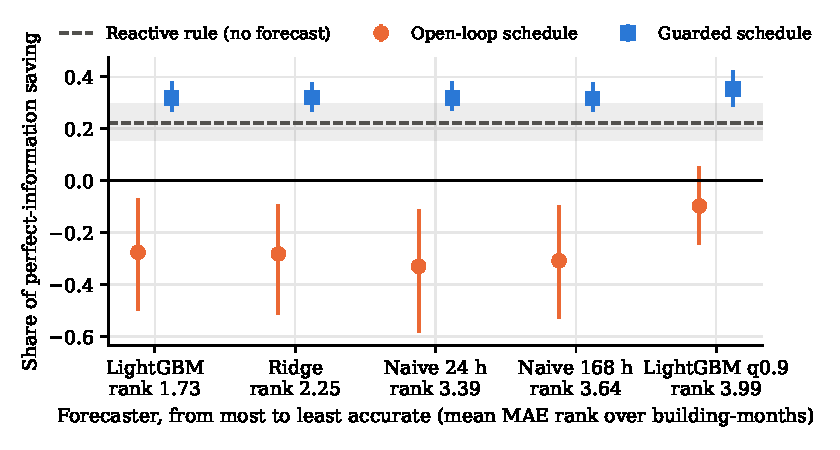
\includegraphics[width=\linewidth]{figures/fig_share_by_forecaster.pdf}
\caption{Annual share of the perfect-information saving under the demand-charge tariff, by forecaster (ordered by mean MAE rank, 1 = most accurate) and controller. Points are medians over \res{nKept} buildings, bars interquartile ranges; the dashed line and band are the median and interquartile range of the forecast-free reactive rule. Negative values mean a higher bill than without a battery.}\label{fig:share}
\end{figure}

Figure~\ref{fig:share} shows the annual captured share by forecaster and controller. Executed open loop, every forecaster had a negative median share, from $\res{shOpenLo}$ to $\res{shOpenHi}$: the battery raised the bill above the no-battery bill in \res{negT1F1}\% (F1), \res{negT1F2}\% (F2), \res{negT1F3}\% (F3), \res{negT1F4}\% (F4) and \res{negT1F5}\% (F5) of buildings. The mechanism is the asymmetry of the demand charge. The schedule charges in the cheap hours before noon to discharge in the expensive afternoon; when the actual load in a charging hour turns out higher than forecast, the charging power is added to it and can set a new monthly peak. A full-power charge at the hour that becomes the month's peak costs $\lambda P$, as much as a perfectly timed full discharge saves, and the energy arbitrage earns far less than that. The reactive rule, which never charges above the month-to-date peak, captured a median share of $\res{shT1reactive}$ and was at least as good as the best open-loop forecaster in \res{hfourShare}\% of buildings (H4, Holm-adjusted $p=\res{holmH4}$).

The guard removes the asymmetry. With guarded execution, no forecaster raised the annual bill in any building, and the median shares ranged from $\res{shGuardLo}$ to $\res{shGuardHi}$, and the best forecaster of each building beat the reactive rule in \res{hfourbBeatPct}\% of buildings (medians $\res{hfourbBest}$ against $\res{hfourbReactive}$; H4b, $p=\res{hfourbP}$). The reactive rule is a lower bound for a well-tuned forecast-free rule: it charges whenever energy is cheap, including on weekends when no expensive hours follow, and because every day starts at half charge it pays for energy that it never uses. Even so, the step from open loop to the guard changed the median share by more than any choice among the five forecasters did under either controller.

\subsection{Which errors matter (H2)}\label{sec:res-errors}

\begin{figure}[t]
\centering
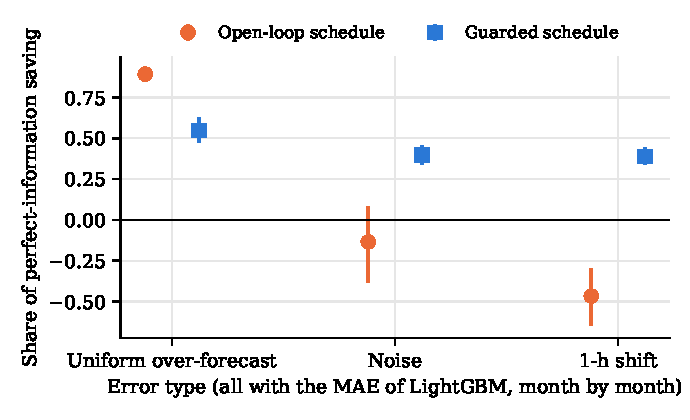
\includegraphics[width=0.78\linewidth]{figures/fig_synthetic.pdf}
\caption{Annual share of the perfect-information saving for three synthetic forecasts with the same MAE as LightGBM in every building-month (medians and interquartile ranges over buildings, demand-charge tariff).}\label{fig:syn}
\end{figure}

The synthetic forecasts isolate the type of error (Figure~\ref{fig:syn}). At the same MAE as F4, a uniform over-forecast kept a median share of $\res{shT1Sscale}$ with open-loop execution, random noise gave $\res{shT1Snoise}$ and a one-hour delay $\res{shT1Sshift}$ (Friedman $p\res{synFriedP}$). With the guard the three were $\res{shT1GSscale}$, $\res{shT1GSnoise}$ and $\res{shT1GSshift}$ (Friedman $p\res{synFriedPg}$): the guard rescues the noisy and late forecasts, and the over-forecast remains the most valuable. Errors that make the forecast load too low at the hours the battery charges are the expensive ones; errors that make it too high are cheap, because they lead the schedule to keep charge in reserve.

\begin{figure}[t]
\centering
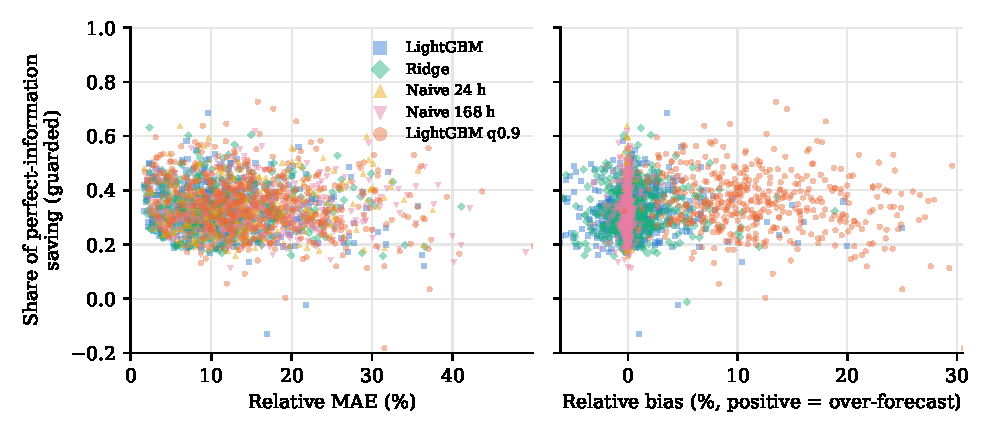
\includegraphics[width=\linewidth]{figures/fig_accuracy_vs_value.pdf}
\caption{Accuracy and bias against value. Each point is a building and forecaster: relative MAE (left) and relative bias (right) over the test year against the annual share of the perfect-information saving with guarded execution (demand-charge tariff).}\label{fig:acc}
\end{figure}

The real forecasters show the same pattern (Figure~\ref{fig:acc}). The 0.9-quantile model F5 was the least accurate on average (mean MAE rank \res{rankF5} of 5 across building-months, last in \res{worstF5}\%, against \res{rankF4} for F4) and the only one with a material bias (\res{relbiasF5}\%), and it captured the largest median share under both controllers (open loop $\res{shT1F5}$, guarded $\res{shT1GF5}$). Across buildings and forecasters, the Spearman correlation of the annual share with accuracy (negative relative MAE) was $\res{rhoMaeOpen}$ for open-loop schedules and $\res{rhoMaeGuard}$ with the guard, and with relative bias $\res{rhoBiasOpen}$ and $\res{rhoBiasGuard}$ (exploratory). The pre-registered H2 asked whether the error of the forecast daily peak predicts value better than the MAE; it did not (mean per-building Spearman correlations $\res{htwoRhoPeak}$ and $\res{htwoRhoMae}$, Holm-adjusted $p=\res{holmH2}$). Both are negative under open loop: the peak magnitude, like the average, is the wrong target when the cost of an error depends on its sign.

\subsection{Without a demand charge, accuracy does not matter (H3)}

Under the time-of-use tariff T2 every forecaster captured the full perfect-information saving: the median annual share was $\res{shT2F1}$ for each of F1--F5 and no building-forecaster pair was below zero. The schedule of a pure arbitrage program depends on the prices, not on the load, as long as the load exceeds the battery's discharge. Kendall's $\tau$ is therefore undefined in most buildings; in the \res{hthreeN} buildings where the shares differed under both tariffs, agreement was higher under T2 than under T1 ($\res{hthreeTauTwo}$ against $\res{hthreeTauOne}$; H3, Holm-adjusted $p=\res{holmH3}$), but the differences it ranks are negligible.

\subsection{Robustness}

\begin{table}[t]
\centering
\footnotesize
\caption{Primary test (H1) under alternative batteries and demand charges: mean per-building Kendall $\tau$ between accuracy (negative MAE) and captured share, open-loop execution unless stated, demand-charge tariff. Excluded: building-month-tariff cells removed by the 0.5\% rule.}\label{tab:rob}
\setlength{\tabcolsep}{4pt}
\begin{tabular}{lrrrr}
\toprule
Setting & Mean $\tau$ & $p$ & $\tau>0$ (\%) & Excluded \\
\midrule
Base: $P$ = 10\% of peak, 20 \$/kW & $\res{honeMean}$ & \res{honeP} & \res{honePos} & \res{nBMexcl} \\
$P$ = 5\% of peak & $\res{robb05Mean}$ & \res{robb05P} & \res{robb05Pos} & \res{robb05Excl} \\
$P$ = 20\% of peak & $\res{robb20Mean}$ & \res{robb20P} & \res{robb20Pos} & \res{robb20Excl} \\
Demand charge 10 \$/kW & $\res{robdc10Mean}$ & \res{robdc10P} & \res{robdc10Pos} & \res{robdc10Excl} \\
Demand charge 30 \$/kW & $\res{robdc30Mean}$ & \res{robdc30P} & \res{robdc30Pos} & \res{robdc30Excl} \\
Base, guarded execution & $\res{honebMean}$ & \res{honebP} & \res{honebPos} & \res{nBMexcl} \\
\bottomrule
\end{tabular}
\end{table}

Table~\ref{tab:rob} repeats the primary test under the pre-listed alternatives. The sign of $\tau$ depends on the battery: slightly positive with a small battery and negative with a large one, which charges harder and so has more to lose from charging into an unforecast peak. In no setting did the mean $\tau$ exceed \res{robMaxAbsTau} in absolute value. Across buildings, the best forecaster's open-loop share was lower in buildings with a high load factor (Spearman $\res{modLF}$) and higher in buildings with more day-to-day variation ($\res{modCV}$).
